\documentclass[twoside]{book}

% Packages required by doxygen
\usepackage{fixltx2e}
\usepackage{calc}
\usepackage{doxygen}
\usepackage[export]{adjustbox} % also loads graphicx
\usepackage{graphicx}
\usepackage[utf8]{inputenc}
\usepackage{makeidx}
\usepackage{multicol}
\usepackage{multirow}
\PassOptionsToPackage{warn}{textcomp}
\usepackage{textcomp}
\usepackage[nointegrals]{wasysym}
\usepackage[table]{xcolor}

% Font selection
\usepackage[T1]{fontenc}
\usepackage[scaled=.90]{helvet}
\usepackage{courier}
\usepackage{amssymb}
\usepackage{sectsty}
\renewcommand{\familydefault}{\sfdefault}
\allsectionsfont{%
  \fontseries{bc}\selectfont%
  \color{darkgray}%
}
\renewcommand{\DoxyLabelFont}{%
  \fontseries{bc}\selectfont%
  \color{darkgray}%
}
\newcommand{\+}{\discretionary{\mbox{\scriptsize$\hookleftarrow$}}{}{}}

% Page & text layout
\usepackage{geometry}
\geometry{%
  a4paper,%
  top=2.5cm,%
  bottom=2.5cm,%
  left=2.5cm,%
  right=2.5cm%
}
\tolerance=750
\hfuzz=15pt
\hbadness=750
\setlength{\emergencystretch}{15pt}
\setlength{\parindent}{0cm}
\setlength{\parskip}{3ex plus 2ex minus 2ex}
\makeatletter
\renewcommand{\paragraph}{%
  \@startsection{paragraph}{4}{0ex}{-1.0ex}{1.0ex}{%
    \normalfont\normalsize\bfseries\SS@parafont%
  }%
}
\renewcommand{\subparagraph}{%
  \@startsection{subparagraph}{5}{0ex}{-1.0ex}{1.0ex}{%
    \normalfont\normalsize\bfseries\SS@subparafont%
  }%
}
\makeatother

% Headers & footers
\usepackage{fancyhdr}
\pagestyle{fancyplain}
\fancyhead[LE]{\fancyplain{}{\bfseries\thepage}}
\fancyhead[CE]{\fancyplain{}{}}
\fancyhead[RE]{\fancyplain{}{\bfseries\leftmark}}
\fancyhead[LO]{\fancyplain{}{\bfseries\rightmark}}
\fancyhead[CO]{\fancyplain{}{}}
\fancyhead[RO]{\fancyplain{}{\bfseries\thepage}}
\fancyfoot[LE]{\fancyplain{}{}}
\fancyfoot[CE]{\fancyplain{}{}}
\fancyfoot[RE]{\fancyplain{}{\bfseries\scriptsize Generated by Doxygen }}
\fancyfoot[LO]{\fancyplain{}{\bfseries\scriptsize Generated by Doxygen }}
\fancyfoot[CO]{\fancyplain{}{}}
\fancyfoot[RO]{\fancyplain{}{}}
\renewcommand{\footrulewidth}{0.4pt}
\renewcommand{\chaptermark}[1]{%
  \markboth{#1}{}%
}
\renewcommand{\sectionmark}[1]{%
  \markright{\thesection\ #1}%
}

% Indices & bibliography
\usepackage{natbib}
\usepackage[titles]{tocloft}
\setcounter{tocdepth}{3}
\setcounter{secnumdepth}{5}
\makeindex

% Hyperlinks (required, but should be loaded last)
\usepackage{ifpdf}
\ifpdf
  \usepackage[pdftex,pagebackref=true]{hyperref}
\else
  \usepackage[ps2pdf,pagebackref=true]{hyperref}
\fi
\hypersetup{%
  colorlinks=true,%
  linkcolor=blue,%
  citecolor=blue,%
  unicode%
}

% Custom commands
\newcommand{\clearemptydoublepage}{%
  \newpage{\pagestyle{empty}\cleardoublepage}%
}

\usepackage{caption}
\captionsetup{labelsep=space,justification=centering,font={bf},singlelinecheck=off,skip=4pt,position=top}

%===== C O N T E N T S =====

\begin{document}

% Titlepage & ToC
\hypersetup{pageanchor=false,
             bookmarksnumbered=true,
             pdfencoding=unicode
            }
\pagenumbering{alph}
\begin{titlepage}
\vspace*{7cm}
\begin{center}%
{\Large Compilation }\\
\vspace*{1cm}
{\large Generated by Doxygen 1.8.13}\\
\end{center}
\end{titlepage}
\clearemptydoublepage
\pagenumbering{roman}
\tableofcontents
\clearemptydoublepage
\pagenumbering{arabic}
\hypersetup{pageanchor=true}

%--- Begin generated contents ---
\chapter{Data Structure Index}
\section{Data Structures}
Here are the data structures with brief descriptions\+:\begin{DoxyCompactList}
\item\contentsline{section}{\hyperlink{structcel}{cel} }{\pageref{structcel}}{}
\item\contentsline{section}{\hyperlink{struct_c_o_n_s_tentry}{C\+O\+N\+S\+Tentry} \\*Define a struct for a constante }{\pageref{struct_c_o_n_s_tentry}}{}
\item\contentsline{section}{\hyperlink{structftable}{ftable} }{\pageref{structftable}}{}
\item\contentsline{section}{\hyperlink{structfun}{fun} }{\pageref{structfun}}{}
\item\contentsline{section}{\hyperlink{struct_m_a_c_r_oentry}{M\+A\+C\+R\+Oentry} \\*Define a struct for a macro constante }{\pageref{struct_m_a_c_r_oentry}}{}
\item\contentsline{section}{\hyperlink{struct_mtable}{Mtable} }{\pageref{struct_mtable}}{}
\item\contentsline{section}{\hyperlink{struct_s_tentry}{S\+Tentry} \\*Define a struct for a variable }{\pageref{struct_s_tentry}}{}
\end{DoxyCompactList}

\chapter{File Index}
\section{File List}
Here is a list of all documented files with brief descriptions\+:\begin{DoxyCompactList}
\item\contentsline{section}{header/\hyperlink{decl_8h}{decl.\+h} \\*Define the stack, Symbol Table of Variables, Constantes, Function }{\pageref{decl_8h}}{}
\end{DoxyCompactList}

\chapter{Data Structure Documentation}
\hypertarget{structcel}{}\section{cel Struct Reference}
\label{structcel}\index{cel@{cel}}


Collaboration diagram for cel\+:\nopagebreak
\begin{figure}[H]
\begin{center}
\leavevmode
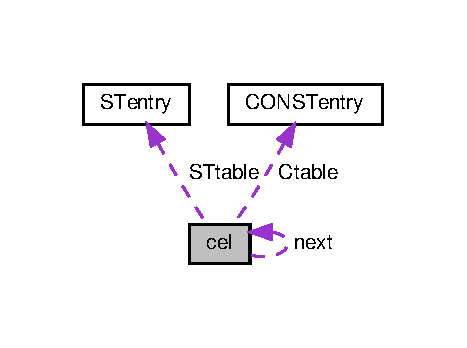
\includegraphics[width=224pt]{structcel__coll__graph}
\end{center}
\end{figure}
\subsection*{Data Fields}
\begin{DoxyCompactItemize}
\item 
\mbox{\Hypertarget{structcel_a6812d40652d2bac79cfa87079b8cb7b9}\label{structcel_a6812d40652d2bac79cfa87079b8cb7b9}} 
\hyperlink{struct_s_tentry}{S\+Tentry} $\ast$ {\bfseries S\+Ttable}
\item 
\mbox{\Hypertarget{structcel_a83cd4ff203668f9dbbed335c25af0d64}\label{structcel_a83cd4ff203668f9dbbed335c25af0d64}} 
\hyperlink{struct_c_o_n_s_tentry}{C\+O\+N\+S\+Tentry} $\ast$ {\bfseries Ctable}
\item 
\mbox{\Hypertarget{structcel_adbb368ad027ec24104f6cd5f7f7d2c0d}\label{structcel_adbb368ad027ec24104f6cd5f7f7d2c0d}} 
int {\bfseries S\+Tmax}
\item 
\mbox{\Hypertarget{structcel_a4a9f95fa763ad7614424fccd9b8d00a6}\label{structcel_a4a9f95fa763ad7614424fccd9b8d00a6}} 
int {\bfseries S\+Tsize}
\item 
\mbox{\Hypertarget{structcel_a708c0152509a4fc390cc7904be927b58}\label{structcel_a708c0152509a4fc390cc7904be927b58}} 
int {\bfseries Cmax}
\item 
\mbox{\Hypertarget{structcel_a64088910a6c1c39223f36d17273377f3}\label{structcel_a64088910a6c1c39223f36d17273377f3}} 
int {\bfseries Csize}
\item 
\mbox{\Hypertarget{structcel_a2f9dadae50a6e7f11a73d87380851be4}\label{structcel_a2f9dadae50a6e7f11a73d87380851be4}} 
int {\bfseries current\+\_\+stack\+\_\+address}
\item 
\mbox{\Hypertarget{structcel_a3ac2fa6ca480a8d2f10024e97a0be547}\label{structcel_a3ac2fa6ca480a8d2f10024e97a0be547}} 
struct \hyperlink{structcel}{cel} $\ast$ {\bfseries next}
\end{DoxyCompactItemize}


The documentation for this struct was generated from the following file\+:\begin{DoxyCompactItemize}
\item 
header/\hyperlink{decl_8h}{decl.\+h}\end{DoxyCompactItemize}

\hypertarget{struct_c_o_n_s_tentry}{}\section{C\+O\+N\+S\+Tentry Struct Reference}
\label{struct_c_o_n_s_tentry}\index{C\+O\+N\+S\+Tentry@{C\+O\+N\+S\+Tentry}}


define a struct for a constante.  




{\ttfamily \#include $<$decl.\+h$>$}

\subsection*{Data Fields}
\begin{DoxyCompactItemize}
\item 
\mbox{\Hypertarget{struct_c_o_n_s_tentry_afdd40a771835cf5f3511c7ac6fb6e664}\label{struct_c_o_n_s_tentry_afdd40a771835cf5f3511c7ac6fb6e664}} 
char {\bfseries name} \mbox{[}M\+A\+X\+N\+A\+ME\mbox{]}
\item 
\mbox{\Hypertarget{struct_c_o_n_s_tentry_ac765329451135abec74c45e1897abf26}\label{struct_c_o_n_s_tentry_ac765329451135abec74c45e1897abf26}} 
int {\bfseries type}
\item 
\mbox{\Hypertarget{struct_c_o_n_s_tentry_ac4f474c82e82cbb89ca7c36dd52be0ed}\label{struct_c_o_n_s_tentry_ac4f474c82e82cbb89ca7c36dd52be0ed}} 
int {\bfseries value}
\item 
\mbox{\Hypertarget{struct_c_o_n_s_tentry_ab271bf689e787edf8ddff375682937d2}\label{struct_c_o_n_s_tentry_ab271bf689e787edf8ddff375682937d2}} 
float {\bfseries value\+Float}
\end{DoxyCompactItemize}


\subsection{Detailed Description}
define a struct for a constante. 

\hyperlink{struct_c_o_n_s_tentry}{C\+O\+N\+S\+Tentry} is a name, a type and a value. 

The documentation for this struct was generated from the following file\+:\begin{DoxyCompactItemize}
\item 
header/\hyperlink{decl_8h}{decl.\+h}\end{DoxyCompactItemize}

\hypertarget{structftable}{}\section{ftable Struct Reference}
\label{structftable}\index{ftable@{ftable}}


Collaboration diagram for ftable\+:\nopagebreak
\begin{figure}[H]
\begin{center}
\leavevmode
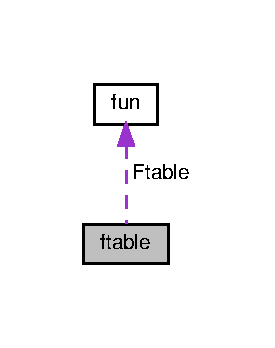
\includegraphics[width=132pt]{structftable__coll__graph}
\end{center}
\end{figure}
\subsection*{Data Fields}
\begin{DoxyCompactItemize}
\item 
\mbox{\Hypertarget{structftable_aca10ea87e4ecbebc41fa08736c462197}\label{structftable_aca10ea87e4ecbebc41fa08736c462197}} 
\hyperlink{structfun}{F\+U\+Nentry} $\ast$ {\bfseries Ftable}
\item 
\mbox{\Hypertarget{structftable_a34c8933e3338d011fd77921cb34ddc61}\label{structftable_a34c8933e3338d011fd77921cb34ddc61}} 
int {\bfseries Fsize}
\item 
\mbox{\Hypertarget{structftable_a38b6b9aaf8c248ce4eee091119712693}\label{structftable_a38b6b9aaf8c248ce4eee091119712693}} 
int {\bfseries Fmax}
\end{DoxyCompactItemize}


The documentation for this struct was generated from the following file\+:\begin{DoxyCompactItemize}
\item 
header/\hyperlink{decl_8h}{decl.\+h}\end{DoxyCompactItemize}

\hypertarget{structfun}{}\section{fun Struct Reference}
\label{structfun}\index{fun@{fun}}
\subsection*{Data Fields}
\begin{DoxyCompactItemize}
\item 
\mbox{\Hypertarget{structfun_afdd40a771835cf5f3511c7ac6fb6e664}\label{structfun_afdd40a771835cf5f3511c7ac6fb6e664}} 
char {\bfseries name} \mbox{[}M\+A\+X\+N\+A\+ME\mbox{]}
\item 
\mbox{\Hypertarget{structfun_a898b215286a6574d95803a8ba019a0ea}\label{structfun_a898b215286a6574d95803a8ba019a0ea}} 
int $\ast$ {\bfseries args}
\item 
\mbox{\Hypertarget{structfun_a7239f4accd8e685ac9d88cb0f1eca6be}\label{structfun_a7239f4accd8e685ac9d88cb0f1eca6be}} 
int {\bfseries Nargs}
\item 
\mbox{\Hypertarget{structfun_a234ea53da5de088dfacb77b9f7a3e7d3}\label{structfun_a234ea53da5de088dfacb77b9f7a3e7d3}} 
int {\bfseries M\+A\+Xargs}
\item 
\mbox{\Hypertarget{structfun_a3a30fedbb952e6b50ccb4f70a75cef05}\label{structfun_a3a30fedbb952e6b50ccb4f70a75cef05}} 
int {\bfseries return\+\_\+type}
\end{DoxyCompactItemize}


The documentation for this struct was generated from the following file\+:\begin{DoxyCompactItemize}
\item 
header/\hyperlink{decl_8h}{decl.\+h}\end{DoxyCompactItemize}

\hypertarget{struct_m_a_c_r_oentry}{}\section{M\+A\+C\+R\+Oentry Struct Reference}
\label{struct_m_a_c_r_oentry}\index{M\+A\+C\+R\+Oentry@{M\+A\+C\+R\+Oentry}}


define a struct for a macro constante.  




{\ttfamily \#include $<$decl.\+h$>$}

\subsection*{Data Fields}
\begin{DoxyCompactItemize}
\item 
\mbox{\Hypertarget{struct_m_a_c_r_oentry_afdd40a771835cf5f3511c7ac6fb6e664}\label{struct_m_a_c_r_oentry_afdd40a771835cf5f3511c7ac6fb6e664}} 
char {\bfseries name} \mbox{[}M\+A\+X\+N\+A\+ME\mbox{]}
\item 
\mbox{\Hypertarget{struct_m_a_c_r_oentry_ac765329451135abec74c45e1897abf26}\label{struct_m_a_c_r_oentry_ac765329451135abec74c45e1897abf26}} 
int {\bfseries type}
\item 
\mbox{\Hypertarget{struct_m_a_c_r_oentry_ac4f474c82e82cbb89ca7c36dd52be0ed}\label{struct_m_a_c_r_oentry_ac4f474c82e82cbb89ca7c36dd52be0ed}} 
int {\bfseries value}
\item 
\mbox{\Hypertarget{struct_m_a_c_r_oentry_ab271bf689e787edf8ddff375682937d2}\label{struct_m_a_c_r_oentry_ab271bf689e787edf8ddff375682937d2}} 
float {\bfseries value\+Float}
\end{DoxyCompactItemize}


\subsection{Detailed Description}
define a struct for a macro constante. 

\hyperlink{struct_m_a_c_r_oentry}{M\+A\+C\+R\+Oentry} is a name, a type and a value. 

The documentation for this struct was generated from the following file\+:\begin{DoxyCompactItemize}
\item 
header/\hyperlink{decl_8h}{decl.\+h}\end{DoxyCompactItemize}

\hypertarget{struct_mtable}{}\section{Mtable Struct Reference}
\label{struct_mtable}\index{Mtable@{Mtable}}


Collaboration diagram for Mtable\+:\nopagebreak
\begin{figure}[H]
\begin{center}
\leavevmode
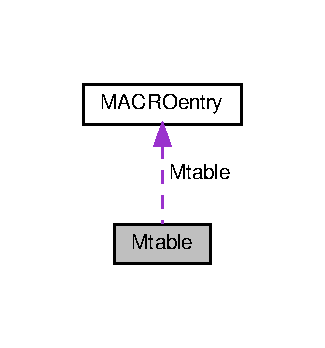
\includegraphics[width=156pt]{struct_mtable__coll__graph}
\end{center}
\end{figure}
\subsection*{Data Fields}
\begin{DoxyCompactItemize}
\item 
\mbox{\Hypertarget{struct_mtable_ad0484a655e4eae46e745aebd6441b135}\label{struct_mtable_ad0484a655e4eae46e745aebd6441b135}} 
\hyperlink{struct_m_a_c_r_oentry}{M\+A\+C\+R\+Oentry} $\ast$ {\bfseries Mtable}
\item 
\mbox{\Hypertarget{struct_mtable_ac6e9569a0a0277558387c0577d73b746}\label{struct_mtable_ac6e9569a0a0277558387c0577d73b746}} 
int {\bfseries Msize}
\item 
\mbox{\Hypertarget{struct_mtable_aa6d3d414d4977af387a63b8563de99d4}\label{struct_mtable_aa6d3d414d4977af387a63b8563de99d4}} 
int {\bfseries Mmax}
\end{DoxyCompactItemize}


The documentation for this struct was generated from the following file\+:\begin{DoxyCompactItemize}
\item 
header/\hyperlink{decl_8h}{decl.\+h}\end{DoxyCompactItemize}

\hypertarget{struct_s_tentry}{}\section{S\+Tentry Struct Reference}
\label{struct_s_tentry}\index{S\+Tentry@{S\+Tentry}}


define a struct for a variable.  




{\ttfamily \#include $<$decl.\+h$>$}

\subsection*{Data Fields}
\begin{DoxyCompactItemize}
\item 
\mbox{\Hypertarget{struct_s_tentry_afdd40a771835cf5f3511c7ac6fb6e664}\label{struct_s_tentry_afdd40a771835cf5f3511c7ac6fb6e664}} 
char {\bfseries name} \mbox{[}M\+A\+X\+N\+A\+ME\mbox{]}
\item 
\mbox{\Hypertarget{struct_s_tentry_ac765329451135abec74c45e1897abf26}\label{struct_s_tentry_ac765329451135abec74c45e1897abf26}} 
int {\bfseries type}
\item 
\mbox{\Hypertarget{struct_s_tentry_a45c6bc6d1135dc398bf8deae861a2ebc}\label{struct_s_tentry_a45c6bc6d1135dc398bf8deae861a2ebc}} 
int {\bfseries address}
\item 
\mbox{\Hypertarget{struct_s_tentry_a439227feff9d7f55384e8780cfc2eb82}\label{struct_s_tentry_a439227feff9d7f55384e8780cfc2eb82}} 
int {\bfseries size}
\item 
\mbox{\Hypertarget{struct_s_tentry_a6ccc3a2456c4631091ce42a637053789}\label{struct_s_tentry_a6ccc3a2456c4631091ce42a637053789}} 
long {\bfseries value}
\item 
\mbox{\Hypertarget{struct_s_tentry_ab271bf689e787edf8ddff375682937d2}\label{struct_s_tentry_ab271bf689e787edf8ddff375682937d2}} 
float {\bfseries value\+Float}
\end{DoxyCompactItemize}


\subsection{Detailed Description}
define a struct for a variable. 

\hyperlink{struct_s_tentry}{S\+Tentry} is a name (ident) with a type, address and size. If the variable isn\textquotesingle{}t an array, the size is null (0). 

The documentation for this struct was generated from the following file\+:\begin{DoxyCompactItemize}
\item 
header/\hyperlink{decl_8h}{decl.\+h}\end{DoxyCompactItemize}

\chapter{File Documentation}
\hypertarget{decl_8h}{}\section{header/decl.h File Reference}
\label{decl_8h}\index{header/decl.\+h@{header/decl.\+h}}


Define the stack, Symbol Table of Variables, Constantes, Function.  


\subsection*{Data Structures}
\begin{DoxyCompactItemize}
\item 
struct \hyperlink{struct_s_tentry}{S\+Tentry}
\begin{DoxyCompactList}\small\item\em define a struct for a variable. \end{DoxyCompactList}\item 
struct \hyperlink{struct_c_o_n_s_tentry}{C\+O\+N\+S\+Tentry}
\begin{DoxyCompactList}\small\item\em define a struct for a constante. \end{DoxyCompactList}\item 
struct \hyperlink{struct_m_a_c_r_oentry}{M\+A\+C\+R\+Oentry}
\begin{DoxyCompactList}\small\item\em define a struct for a macro constante. \end{DoxyCompactList}\item 
struct \hyperlink{struct_mtable}{Mtable}
\item 
struct \hyperlink{structcel}{cel}
\item 
struct \hyperlink{structfun}{fun}
\item 
struct \hyperlink{structftable}{ftable}
\end{DoxyCompactItemize}
\subsection*{Macros}
\begin{DoxyCompactItemize}
\item 
\mbox{\Hypertarget{decl_8h_a3da44afeba217135a680a7477b5e3ce3}\label{decl_8h_a3da44afeba217135a680a7477b5e3ce3}} 
\#define {\bfseries D\+E\+F\+A\+U\+LT}~\char`\"{}\textbackslash{}033\mbox{[}0m\char`\"{}
\item 
\mbox{\Hypertarget{decl_8h_ab814d2aa388b74d504673d0068cab196}\label{decl_8h_ab814d2aa388b74d504673d0068cab196}} 
\#define {\bfseries H\+I\+G\+H\+L\+I\+G\+HT}~\char`\"{}\textbackslash{}033\mbox{[}1m\char`\"{}
\item 
\mbox{\Hypertarget{decl_8h_aaec1a65734e33bc49e8dc8d90e9546bc}\label{decl_8h_aaec1a65734e33bc49e8dc8d90e9546bc}} 
\#define {\bfseries U\+N\+D\+E\+R\+L\+I\+NE}~\char`\"{}\textbackslash{}033\mbox{[}4m\char`\"{}
\item 
\mbox{\Hypertarget{decl_8h_a38eec52a7dccb94ff563e30eda32c891}\label{decl_8h_a38eec52a7dccb94ff563e30eda32c891}} 
\#define {\bfseries B\+L\+I\+NK}~\char`\"{}\textbackslash{}033\mbox{[}5m\char`\"{}
\item 
\mbox{\Hypertarget{decl_8h_a7b3b25cba33b07c303f3060fe41887f6}\label{decl_8h_a7b3b25cba33b07c303f3060fe41887f6}} 
\#define {\bfseries B\+L\+A\+CK}~\char`\"{}\textbackslash{}033\mbox{[}30m\char`\"{}
\item 
\mbox{\Hypertarget{decl_8h_a8d23feea868a983c8c2b661e1e16972f}\label{decl_8h_a8d23feea868a983c8c2b661e1e16972f}} 
\#define {\bfseries R\+ED}~\char`\"{}\textbackslash{}033\mbox{[}31m\char`\"{}
\item 
\mbox{\Hypertarget{decl_8h_acfbc006ea433ad708fdee3e82996e721}\label{decl_8h_acfbc006ea433ad708fdee3e82996e721}} 
\#define {\bfseries G\+R\+E\+EN}~\char`\"{}\textbackslash{}033\mbox{[}32m\char`\"{}
\item 
\mbox{\Hypertarget{decl_8h_abf681265909adf3d3e8116c93c0ba179}\label{decl_8h_abf681265909adf3d3e8116c93c0ba179}} 
\#define {\bfseries Y\+E\+L\+L\+OW}~\char`\"{}\textbackslash{}033\mbox{[}33m\char`\"{}
\item 
\mbox{\Hypertarget{decl_8h_a79d10e672abb49ad63eeaa8aaef57c38}\label{decl_8h_a79d10e672abb49ad63eeaa8aaef57c38}} 
\#define {\bfseries B\+L\+UE}~\char`\"{}\textbackslash{}033\mbox{[}34m\char`\"{}
\item 
\mbox{\Hypertarget{decl_8h_a0bb0b009e7a7390473ace4d98bd843c0}\label{decl_8h_a0bb0b009e7a7390473ace4d98bd843c0}} 
\#define {\bfseries P\+U\+R\+P\+LE}~\char`\"{}\textbackslash{}033\mbox{[}35m\char`\"{}
\item 
\mbox{\Hypertarget{decl_8h_ad243f93c16bc4c1d3e0a13b84421d760}\label{decl_8h_ad243f93c16bc4c1d3e0a13b84421d760}} 
\#define {\bfseries C\+Y\+AN}~\char`\"{}\textbackslash{}033\mbox{[}36m\char`\"{}
\item 
\mbox{\Hypertarget{decl_8h_a87b537f5fa5c109d3c05c13d6b18f382}\label{decl_8h_a87b537f5fa5c109d3c05c13d6b18f382}} 
\#define {\bfseries W\+H\+I\+TE}~\char`\"{}\textbackslash{}033\mbox{[}37m\char`\"{}
\item 
\mbox{\Hypertarget{decl_8h_ac881f02a50b29d3ffa5b1f4a0e4f9568}\label{decl_8h_ac881f02a50b29d3ffa5b1f4a0e4f9568}} 
\#define {\bfseries M\+A\+X\+N\+A\+ME}~64
\item 
\mbox{\Hypertarget{decl_8h_ab4c7828c930d89cd887129e2cad38d15}\label{decl_8h_ab4c7828c930d89cd887129e2cad38d15}} 
\#define {\bfseries M\+A\+X\+N\+B\+S\+Y\+M\+B\+OL}~32
\item 
\mbox{\Hypertarget{decl_8h_a9d7fd488d95e6c91df3e0e4b02516925}\label{decl_8h_a9d7fd488d95e6c91df3e0e4b02516925}} 
\#define {\bfseries E\+R\+R\+\_\+\+T\+Y\+PE}~-\/1
\item 
\mbox{\Hypertarget{decl_8h_a35cd67ba7bb0db8105eb6267467535d7}\label{decl_8h_a35cd67ba7bb0db8105eb6267467535d7}} 
\#define {\bfseries C\+H\+AR}~0
\item 
\mbox{\Hypertarget{decl_8h_a91d43eadec33c80149f92e5abf5df58c}\label{decl_8h_a91d43eadec33c80149f92e5abf5df58c}} 
\#define {\bfseries I\+N\+T\+E\+G\+ER}~1
\item 
\mbox{\Hypertarget{decl_8h_a4b654506f18b8bfd61ad2a29a7e38c25}\label{decl_8h_a4b654506f18b8bfd61ad2a29a7e38c25}} 
\#define {\bfseries R\+E\+AL}~2
\item 
\mbox{\Hypertarget{decl_8h_a75bfd14b4b0ebac12ba08b9b36229225}\label{decl_8h_a75bfd14b4b0ebac12ba08b9b36229225}} 
\#define {\bfseries V\+O\+I\+D\+T\+Y\+PE}~3
\item 
\mbox{\Hypertarget{decl_8h_acaa7b8a7167a8214f499c71c413ddcca}\label{decl_8h_acaa7b8a7167a8214f499c71c413ddcca}} 
\#define {\bfseries L\+O\+NG}~4
\end{DoxyCompactItemize}
\subsection*{Typedefs}
\begin{DoxyCompactItemize}
\item 
\mbox{\Hypertarget{decl_8h_abd357765dc59dbe80107e9b364e88423}\label{decl_8h_abd357765dc59dbe80107e9b364e88423}} 
typedef struct \hyperlink{structcel}{cel} {\bfseries S\+T\+Stack\+Cel}
\item 
\mbox{\Hypertarget{decl_8h_a280200a32c878643be7cca2a261ff0e9}\label{decl_8h_a280200a32c878643be7cca2a261ff0e9}} 
typedef struct \hyperlink{structcel}{cel} $\ast$ {\bfseries S\+T\+Stack}
\item 
\mbox{\Hypertarget{decl_8h_aa4ecefb2487498d22b878ceef41644dc}\label{decl_8h_aa4ecefb2487498d22b878ceef41644dc}} 
typedef struct \hyperlink{structfun}{fun} {\bfseries F\+U\+Nentry}
\item 
\mbox{\Hypertarget{decl_8h_a1b0009df191170a3655b025267557883}\label{decl_8h_a1b0009df191170a3655b025267557883}} 
typedef struct \hyperlink{structftable}{ftable} {\bfseries Ftable}
\end{DoxyCompactItemize}
\subsection*{Functions}
\begin{DoxyCompactItemize}
\item 
\mbox{\Hypertarget{decl_8h_a9d46438ded8523a23a2f6088d282005d}\label{decl_8h_a9d46438ded8523a23a2f6088d282005d}} 
void \hyperlink{decl_8h_a9d46438ded8523a23a2f6088d282005d}{init\+Prog} ()
\begin{DoxyCompactList}\small\item\em Initialize the programm. \end{DoxyCompactList}\item 
\mbox{\Hypertarget{decl_8h_a7e1f093f0f3c4df44a5c36a418d227d1}\label{decl_8h_a7e1f093f0f3c4df44a5c36a418d227d1}} 
void \hyperlink{decl_8h_a7e1f093f0f3c4df44a5c36a418d227d1}{create\+Stack} ()
\begin{DoxyCompactList}\small\item\em Create the stack. \end{DoxyCompactList}\item 
int \hyperlink{decl_8h_a0640a823bf6808b49b17c76dca5e507e}{get\+Type} (const char $\ast$type)
\begin{DoxyCompactList}\small\item\em return the integer associated to the type. \end{DoxyCompactList}\item 
\mbox{\Hypertarget{decl_8h_a7859abb31b52f3103bf9abfbf308b5de}\label{decl_8h_a7859abb31b52f3103bf9abfbf308b5de}} 
int {\bfseries add\+Var} (const char name\mbox{[}$\,$\mbox{]}, int type, int is\+\_\+parameter, int value, float value\+Float)
\item 
\mbox{\Hypertarget{decl_8h_a540704b40e68f8d3f231feaf5e0658b6}\label{decl_8h_a540704b40e68f8d3f231feaf5e0658b6}} 
int {\bfseries add\+Const} (const char name\mbox{[}$\,$\mbox{]}, int type, int value, float value\+Float)
\item 
int \hyperlink{decl_8h_a6d8698ce57275648d7532e8c50a3fb64}{add\+Macro} (const char name\mbox{[}$\,$\mbox{]}, int type, int value, float value\+Float)
\item 
int \hyperlink{decl_8h_a0cfd69649a4d5c59042257a9629c2373}{add\+Fun} (const char name\mbox{[}$\,$\mbox{]}, int type)
\item 
int \hyperlink{decl_8h_afbb87f6560b8a047bd0049c81c5962c7}{is\+Constante} (const char name\mbox{[}$\,$\mbox{]})
\item 
\mbox{\Hypertarget{decl_8h_a4174cee842087aa601d9a6edf47a84c1}\label{decl_8h_a4174cee842087aa601d9a6edf47a84c1}} 
void \hyperlink{decl_8h_a4174cee842087aa601d9a6edf47a84c1}{display\+Table} ()
\begin{DoxyCompactList}\small\item\em display the table of variables \end{DoxyCompactList}\item 
\mbox{\Hypertarget{decl_8h_a43cc1d28d0a538cf46fadb189659ab8e}\label{decl_8h_a43cc1d28d0a538cf46fadb189659ab8e}} 
void \hyperlink{decl_8h_a43cc1d28d0a538cf46fadb189659ab8e}{display\+Const} ()
\begin{DoxyCompactList}\small\item\em display the table of constantes \end{DoxyCompactList}\item 
\mbox{\Hypertarget{decl_8h_a8b216eeb7d702e8751048150c280b093}\label{decl_8h_a8b216eeb7d702e8751048150c280b093}} 
void \hyperlink{decl_8h_a8b216eeb7d702e8751048150c280b093}{display\+Macro} ()
\begin{DoxyCompactList}\small\item\em display the table of macros \end{DoxyCompactList}\item 
\mbox{\Hypertarget{decl_8h_a49167802cc8892040f20933700161d4f}\label{decl_8h_a49167802cc8892040f20933700161d4f}} 
void \hyperlink{decl_8h_a49167802cc8892040f20933700161d4f}{display\+Fun\+Table} ()
\begin{DoxyCompactList}\small\item\em display the table of functions \end{DoxyCompactList}\item 
int \hyperlink{decl_8h_ad359e9a76208ccba6420396d17c57302}{lookup} (const char name\mbox{[}$\,$\mbox{]}, int is\+\_\+tab)
\begin{DoxyCompactList}\small\item\em verify if a variable or a constante with the same name exists. \end{DoxyCompactList}\item 
int \hyperlink{decl_8h_a8dd04d8de660b650b2744a4048577aeb}{lookup\+Function} (const char name\mbox{[}$\,$\mbox{]})
\begin{DoxyCompactList}\small\item\em verify if a function with the same name exists and return its type. \end{DoxyCompactList}\item 
int \hyperlink{decl_8h_a930b8808372a3d23ee89e16d7cf77b1a}{check\+\_\+types} (int a, int b)
\begin{DoxyCompactList}\small\item\em verify if a and b is the same type. \end{DoxyCompactList}\item 
\mbox{\Hypertarget{decl_8h_af280f9c58161ce866dfe60066ad33711}\label{decl_8h_af280f9c58161ce866dfe60066ad33711}} 
int {\bfseries max\+\_\+type} (int a, int b)
\item 
int \hyperlink{decl_8h_affd8b5fa98fcd03d6d1f4217b7277879}{cast\+\_\+type} (int a, int b, int flag\+\_\+cast)
\item 
void \hyperlink{decl_8h_a73f7f17a31a1bc68a95927fdfcb6d56f}{add\+Arg} (char name\mbox{[}$\,$\mbox{]}, int type)
\item 
\mbox{\Hypertarget{decl_8h_ae6c91966402f3ab76665669d99bf665d}\label{decl_8h_ae6c91966402f3ab76665669d99bf665d}} 
void \hyperlink{decl_8h_ae6c91966402f3ab76665669d99bf665d}{free\+Stack} ()
\begin{DoxyCompactList}\small\item\em free the memory used for the stack \end{DoxyCompactList}\end{DoxyCompactItemize}
\subsection*{Variables}
\begin{DoxyCompactItemize}
\item 
\mbox{\Hypertarget{decl_8h_a7661b5d028be7f8997cef563e3890fd9}\label{decl_8h_a7661b5d028be7f8997cef563e3890fd9}} 
int {\bfseries line\+\_\+num}
\end{DoxyCompactItemize}


\subsection{Detailed Description}
Define the stack, Symbol Table of Variables, Constantes, Function. 

\begin{DoxyAuthor}{Author}
S\+AM Nensy, S\+I\+M\+O\+N\+N\+OT Florent 
\end{DoxyAuthor}
\begin{DoxyVersion}{Version}
1.\+0 
\end{DoxyVersion}
\begin{DoxyDate}{Date}
23rd March 2019 
\end{DoxyDate}


\subsection{Function Documentation}
\mbox{\Hypertarget{decl_8h_a73f7f17a31a1bc68a95927fdfcb6d56f}\label{decl_8h_a73f7f17a31a1bc68a95927fdfcb6d56f}} 
\index{decl.\+h@{decl.\+h}!add\+Arg@{add\+Arg}}
\index{add\+Arg@{add\+Arg}!decl.\+h@{decl.\+h}}
\subsubsection{\texorpdfstring{add\+Arg()}{addArg()}}
{\footnotesize\ttfamily void add\+Arg (\begin{DoxyParamCaption}\item[{char}]{name\mbox{[}$\,$\mbox{]},  }\item[{int}]{type }\end{DoxyParamCaption})}


\begin{DoxyParams}{Parameters}
{\em name} & the name of function use this argument \\
\hline
{\em type} & the type of argument we want add. \\
\hline
\end{DoxyParams}
\mbox{\Hypertarget{decl_8h_a0cfd69649a4d5c59042257a9629c2373}\label{decl_8h_a0cfd69649a4d5c59042257a9629c2373}} 
\index{decl.\+h@{decl.\+h}!add\+Fun@{add\+Fun}}
\index{add\+Fun@{add\+Fun}!decl.\+h@{decl.\+h}}
\subsubsection{\texorpdfstring{add\+Fun()}{addFun()}}
{\footnotesize\ttfamily int add\+Fun (\begin{DoxyParamCaption}\item[{const char}]{name\mbox{[}$\,$\mbox{]},  }\item[{int}]{type }\end{DoxyParamCaption})}


\begin{DoxyParams}{Parameters}
{\em name} & the name of function \\
\hline
{\em type} & the type of return value of function \\
\hline
\end{DoxyParams}
\begin{DoxyReturn}{Returns}
1 if we add the function. 0 else. 
\end{DoxyReturn}
\mbox{\Hypertarget{decl_8h_a6d8698ce57275648d7532e8c50a3fb64}\label{decl_8h_a6d8698ce57275648d7532e8c50a3fb64}} 
\index{decl.\+h@{decl.\+h}!add\+Macro@{add\+Macro}}
\index{add\+Macro@{add\+Macro}!decl.\+h@{decl.\+h}}
\subsubsection{\texorpdfstring{add\+Macro()}{addMacro()}}
{\footnotesize\ttfamily int add\+Macro (\begin{DoxyParamCaption}\item[{const char}]{name\mbox{[}$\,$\mbox{]},  }\item[{int}]{type,  }\item[{int}]{value,  }\item[{float}]{value\+Float }\end{DoxyParamCaption})}


\begin{DoxyParams}{Parameters}
{\em name} & the name of the macro \\
\hline
{\em type} & the type of the macro \\
\hline
{\em value} & the value of the macro \\
\hline
{\em value\+Float} & the float value of the macro \\
\hline
\end{DoxyParams}
\begin{DoxyReturn}{Returns}
1 if we add the macro. 0 else. 
\end{DoxyReturn}
\mbox{\Hypertarget{decl_8h_affd8b5fa98fcd03d6d1f4217b7277879}\label{decl_8h_affd8b5fa98fcd03d6d1f4217b7277879}} 
\index{decl.\+h@{decl.\+h}!cast\+\_\+type@{cast\+\_\+type}}
\index{cast\+\_\+type@{cast\+\_\+type}!decl.\+h@{decl.\+h}}
\subsubsection{\texorpdfstring{cast\+\_\+type()}{cast\_type()}}
{\footnotesize\ttfamily int cast\+\_\+type (\begin{DoxyParamCaption}\item[{int}]{a,  }\item[{int}]{b,  }\item[{int}]{flag\+\_\+cast }\end{DoxyParamCaption})}


\begin{DoxyParams}{Parameters}
{\em a} & the first type \\
\hline
{\em b} & the second type \\
\hline
{\em flag\+\_\+cast} & negatif if we don\textquotesingle{}t use a cast. Else the value of the type use in the cast. \\
\hline
\end{DoxyParams}
\begin{DoxyReturn}{Returns}
the valuation\textquotesingle{}s type of expression. 
\end{DoxyReturn}
\mbox{\Hypertarget{decl_8h_a930b8808372a3d23ee89e16d7cf77b1a}\label{decl_8h_a930b8808372a3d23ee89e16d7cf77b1a}} 
\index{decl.\+h@{decl.\+h}!check\+\_\+types@{check\+\_\+types}}
\index{check\+\_\+types@{check\+\_\+types}!decl.\+h@{decl.\+h}}
\subsubsection{\texorpdfstring{check\+\_\+types()}{check\_types()}}
{\footnotesize\ttfamily int check\+\_\+types (\begin{DoxyParamCaption}\item[{int}]{a,  }\item[{int}]{b }\end{DoxyParamCaption})}



verify if a and b is the same type. 


\begin{DoxyParams}{Parameters}
{\em a} & -\/ the first type \\
\hline
{\em b} & -\/ the second type \\
\hline
\end{DoxyParams}
\begin{DoxyReturn}{Returns}
1 if a and b is the same type. 0 else. 
\end{DoxyReturn}
\mbox{\Hypertarget{decl_8h_a0640a823bf6808b49b17c76dca5e507e}\label{decl_8h_a0640a823bf6808b49b17c76dca5e507e}} 
\index{decl.\+h@{decl.\+h}!get\+Type@{get\+Type}}
\index{get\+Type@{get\+Type}!decl.\+h@{decl.\+h}}
\subsubsection{\texorpdfstring{get\+Type()}{getType()}}
{\footnotesize\ttfamily int get\+Type (\begin{DoxyParamCaption}\item[{const char $\ast$}]{type }\end{DoxyParamCaption})}



return the integer associated to the type. 


\begin{DoxyParams}{Parameters}
{\em type} & -\/ a string which is a type (int, char, long, float...) \\
\hline
\end{DoxyParams}
\begin{DoxyReturn}{Returns}
the Macro\+Type. 
\end{DoxyReturn}
\mbox{\Hypertarget{decl_8h_afbb87f6560b8a047bd0049c81c5962c7}\label{decl_8h_afbb87f6560b8a047bd0049c81c5962c7}} 
\index{decl.\+h@{decl.\+h}!is\+Constante@{is\+Constante}}
\index{is\+Constante@{is\+Constante}!decl.\+h@{decl.\+h}}
\subsubsection{\texorpdfstring{is\+Constante()}{isConstante()}}
{\footnotesize\ttfamily is\+Constante (\begin{DoxyParamCaption}\item[{const char}]{name\mbox{[}$\,$\mbox{]} }\end{DoxyParamCaption})}


\begin{DoxyParams}{Parameters}
{\em name} & the name of variable, constante, macro we want check. \\
\hline
\end{DoxyParams}
\begin{DoxyReturn}{Returns}
1 if this is a constante. 0 else. 
\end{DoxyReturn}
\mbox{\Hypertarget{decl_8h_ad359e9a76208ccba6420396d17c57302}\label{decl_8h_ad359e9a76208ccba6420396d17c57302}} 
\index{decl.\+h@{decl.\+h}!lookup@{lookup}}
\index{lookup@{lookup}!decl.\+h@{decl.\+h}}
\subsubsection{\texorpdfstring{lookup()}{lookup()}}
{\footnotesize\ttfamily int lookup (\begin{DoxyParamCaption}\item[{const char}]{name\mbox{[}$\,$\mbox{]},  }\item[{int}]{is\+\_\+tab }\end{DoxyParamCaption})}



verify if a variable or a constante with the same name exists. 


\begin{DoxyParams}{Parameters}
{\em name} & -\/ the name of the ident we want check \\
\hline
{\em is\+\_\+tab} & -\/ 0 if this is a variable, else the size of the array. \\
\hline
\end{DoxyParams}
\begin{DoxyReturn}{Returns}
the type of the variable or constante in the stack with this name. Else -\/1. 
\end{DoxyReturn}
\mbox{\Hypertarget{decl_8h_a8dd04d8de660b650b2744a4048577aeb}\label{decl_8h_a8dd04d8de660b650b2744a4048577aeb}} 
\index{decl.\+h@{decl.\+h}!lookup\+Function@{lookup\+Function}}
\index{lookup\+Function@{lookup\+Function}!decl.\+h@{decl.\+h}}
\subsubsection{\texorpdfstring{lookup\+Function()}{lookupFunction()}}
{\footnotesize\ttfamily int lookup\+Function (\begin{DoxyParamCaption}\item[{const char}]{name\mbox{[}$\,$\mbox{]} }\end{DoxyParamCaption})}



verify if a function with the same name exists and return its type. 


\begin{DoxyParams}{Parameters}
{\em name} & -\/ the name of the function we want check\\
\hline
\end{DoxyParams}
\begin{DoxyReturn}{Returns}
the type of the function with this name in the stack. Else -\/1. 
\end{DoxyReturn}

%--- End generated contents ---

% Index
\backmatter
\newpage
\phantomsection
\clearemptydoublepage
\addcontentsline{toc}{chapter}{Index}
\printindex

\end{document}
